\documentclass[journal,11pt]{IEEEtran}
\usepackage{setspace}
\usepackage{gensymb}
\singlespacing
\usepackage[cmex10]{amsmath}
\usepackage{amsthm}
\usepackage{mathrsfs}
\usepackage{txfonts}
\usepackage{stfloats}
\usepackage{bm}
\usepackage{cite}
\usepackage{cases}
\usepackage{subfig}
\usepackage{longtable}
\usepackage{multirow}
\usepackage{enumitem}
\usepackage{mathtools}
\usepackage{tikz}
\usepackage{circuitikz}
\usepackage{verbatim}
\usepackage[breaklinks=true]{hyperref}
\usepackage{tkz-euclide} % loads  TikZ and tkz-base
\usepackage{listings}
\usepackage{color}    
\usepackage{array}    
\usepackage{longtable}
\usepackage{calc}     
\usepackage{multirow} 
\usepackage{hhline}   
\usepackage{ifthen}   
\usepackage{lscape}     
\usepackage{chngcntr}
\usepackage{float}
\usepackage{gvv}

\begin{document}

\vspace{3cm}
\author{Ajay Krishnan K\\EE22BTECH11003}

\title{Gate ST-37.2023}
\maketitle

\textbf{Question}
\begin{enumerate}
    \item Let $X$ be a random variable with probability density function
          \begin{align}\
              f(x) = \begin{cases}
                         \frac{1}{x^2} & if x \geq 1 \\
                         0             & otherwise.
                     \end{cases}
          \end{align}
          If $Y = \log_e X$, then $\pr{Y<1 | Y<2 }$ equals


          \solution
          Given, the probability density function of $X$ is
          \begin{align}
              f(x) = \begin{cases}
                         \frac{1}{x^2} & if x \geq 1 \\
                         0             & otherwise.
                     \end{cases}
          \end{align}
          Also, $Y = \log_e X$.\\
          Consider the cumulative distribution function(CDF) of $X$,
          \begin{align}
              F_X(x) & = \pr{X \leq x}                 \\
                     & = \int_{1}^{x} \frac{1}{x^2} dx \\
                     & = 1 - \frac{1}{x} , x \geq 1
          \end{align}
          Now, we need to find the CDF of $Y$.
          \begin{align}
              F_Y(y) & = \pr{Y \leq y}                \\
                     & = \pr{\log_e X \leq y}         \\
                     & = \pr{X \leq e^y}              \\
                     & = F_X(e^y)                     \\
                     & = 1 - \frac{1}{e^y} , y \geq 0
          \end{align}
          \begin{figure}[!ht]
              \centering
              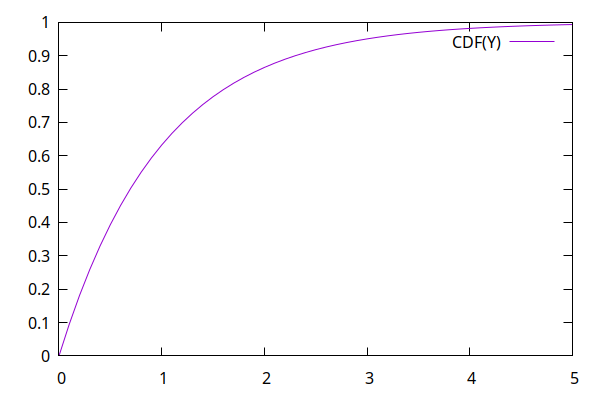
\includegraphics[width=\columnwidth]{./figs/cdf_plot.png}
              \caption{CDF of $Y$}
              \label{fig:cdf_plot}
          \end{figure}


          Now, we need to find $\pr{Y<1 | Y<2 }$.
          For that, we need to find $F_Y(1)$ and $F_Y(2)$.\\
          Using the equation for CDF,
          \begin{align}
              F_Y(1) & = 1 - \frac{1}{e}
          \end{align}
          and
          \begin{align}
              F_Y(2) & = 1 - \frac{1}{e^2}
          \end{align}
          Now, we can find $\pr{Y<1 | Y<2 }$ as follows,
          \begin{align}
              \pr{Y<1 | Y<2 } & = \frac{\pr{Y<1 , Y<2}}{\pr{Y<2}}           \\
                              & = \frac{\pr{Y<1}}{\pr{Y<2}}                 \\
                              & = \frac{F_Y(1)}{F_Y(2)}                     \\
                              & = \frac{1 - \frac{1}{e}}{1 - \frac{1}{e^2}} \\
                              & = \frac{e(e-1)}{e^2-1}                      \\
                              & = \frac{e}{e+1}
          \end{align}

    \item Steps to plot the cdf of $Y$.
          \begin{enumerate}
              \item Generate a uniform random variable between 0 and 1.
              \item Given the PDF of $X$ as $\frac{1}{x^2}$, use the inverse transform method to generate $X$.\\
                    The inverse transform method is given by,
                    \begin{align}
                        X = F^{-1}(U)
                    \end{align}
                    where $U$ is a uniform random variable between 0 and 1 and $F^{-1}$ is the inverse of CDF of $X$.
              \item The CDF of $X$ is given by,
                    \begin{align}
                        F(x) = \int_{1}^{x} \frac{1}{x^2} dx = 1 - \frac{1}{x}
                    \end{align}
              The inverse of CDF of $X$ is given by,
                    \begin{align}
                        F^{-1}(x) = \frac{1}{1-x}
                    \end{align}
              \item Use $X$ to generate $Y = \log_e X$.
              \item Calculate the CDF of $Y$ using the equation $1-\frac{1}{e^y}$.
              \item Store the values of CDF in data file.
              \item Plot the CDF using GNUPlot.
          \end{enumerate}
\end{enumerate}
\end{document}
